\documentclass[svgnames,11pt]{beamer}
\input{/home/tof/Documents/Cozy/latex-include/preambule_commun.tex}
\input{/home/tof/Documents/Cozy/latex-include/preambule_beamer.tex}
%\usepackage{pgfpages} \setbeameroption{show notes on second screen=left}
\author[]{Christophe Viroulaud}
\title{Routing Information Protocol}
\date{\framebox{\textbf{Archi 11}}}
%\logo{}
\institute{Terminale - NSI}

\begin{document}
\begin{frame}
\titlepage
\end{frame}
\begin{frame}
    \frametitle{}

    \begin{center}
    \centering
    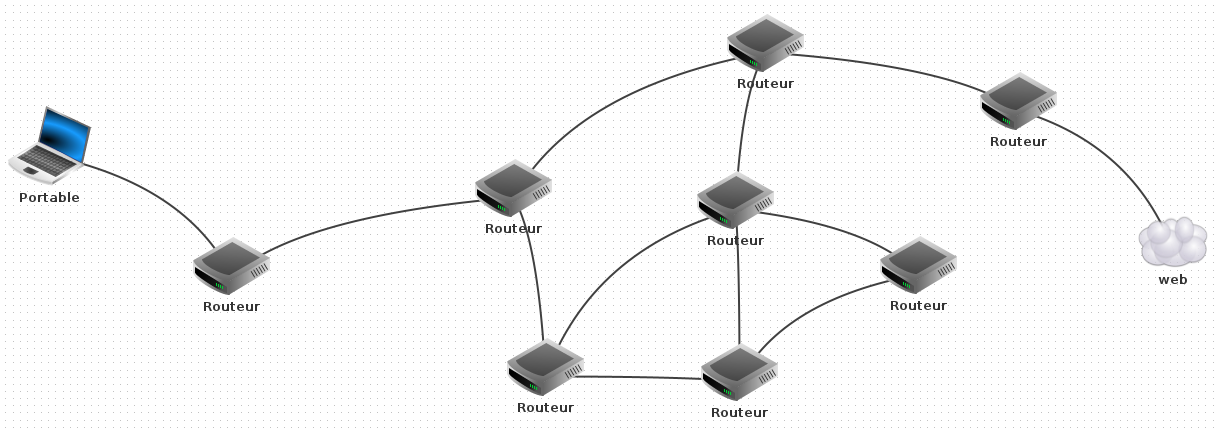
\includegraphics[width=8cm]{ressources/reseau-intro.png}
    \captionof{figure}{Les paquets d'informations se déplacent de routeurs en routeurs.}
    \label{IMG}
    \end{center}

\end{frame}
\begin{frame}
    \frametitle{}

\begin{framed}
    \centering Comment un routeur détermine la route à choisir?
\end{framed}
\end{frame}
\section{Protocole de routage}
\subsection{Principe}
\begin{frame}
    \frametitle{Protocole de routage - principe}
    En plus des paquets, les routeurs s’échangent des informations sur la topologie du réseau.
    \begin{aretenir}[]
        Chaque routeur applique les mêmes règles de communication et de description : c’est le protocole de routage.
    \end{aretenir}

\end{frame}
\begin{frame}
    \frametitle{}

    Il existe plusieurs protocoles:
    \begin{itemize}
        \item \textbf{RIP (Routing Information Protocol): } années 80
        \item \textbf{OSPF (Open Shortest Path First): } fin années 80
        \item \textbf{BGP (Border Gateway Protocol): } fin années 80
    \end{itemize}

\end{frame}
\subsection{Routing Information Protocol}

\begin{frame}
    \frametitle{Routing Information Protocol}

    \begin{aretenir}[]
        Le protocole RIP échange des vecteurs de distance (couple adresse/distance) avec ses routeurs voisins. L’objectif du protocole RIP est de minimiser le nombre de sauts pour atteindre la destination.
    \end{aretenir}

\end{frame}
\begin{frame}

    À intervalle régulier (30 secondes par défaut), chaque routeur transmet à ses voisins:
    \begin{itemize}
        \item<1-> les adresses de ses propres voisins,
        \item<2-> celles qu’il a reçues par d’autres routeurs.
        \item<3-> Il précise également la distance (en
        nombre de sauts) pour atteindre une machine donnée.
    \end{itemize}

\end{frame}
\section{Table de routage}
\subsection{Rôle}
\begin{frame}
    \frametitle{Table de routage - rôle}
\begin{center}
        Chaque routeur construit une table de routage. Elle contient les informations des routes à suivre pour atteindre les autres réseaux.
\end{center}
    

\end{frame}
\begin{frame}
    \frametitle{}

    Chaque ligne de la table de routage contient quatre informations:
\begin{itemize}
    \item<1-> la \emph{destination} sous la forme adresse de sous-réseau/masque,
    \item<2-> la \emph{passerelle} est l'adresse IP du prochain routeur à traverser,
    \item<3-> l'\emph{interface} réseau à utiliser pour rejoindre la passerelle,
    \item<4-> la \emph{distance} vers la destination.
\end{itemize}

\end{frame}
\subsection{Construction}
\begin{frame}
    \frametitle{Construction}
    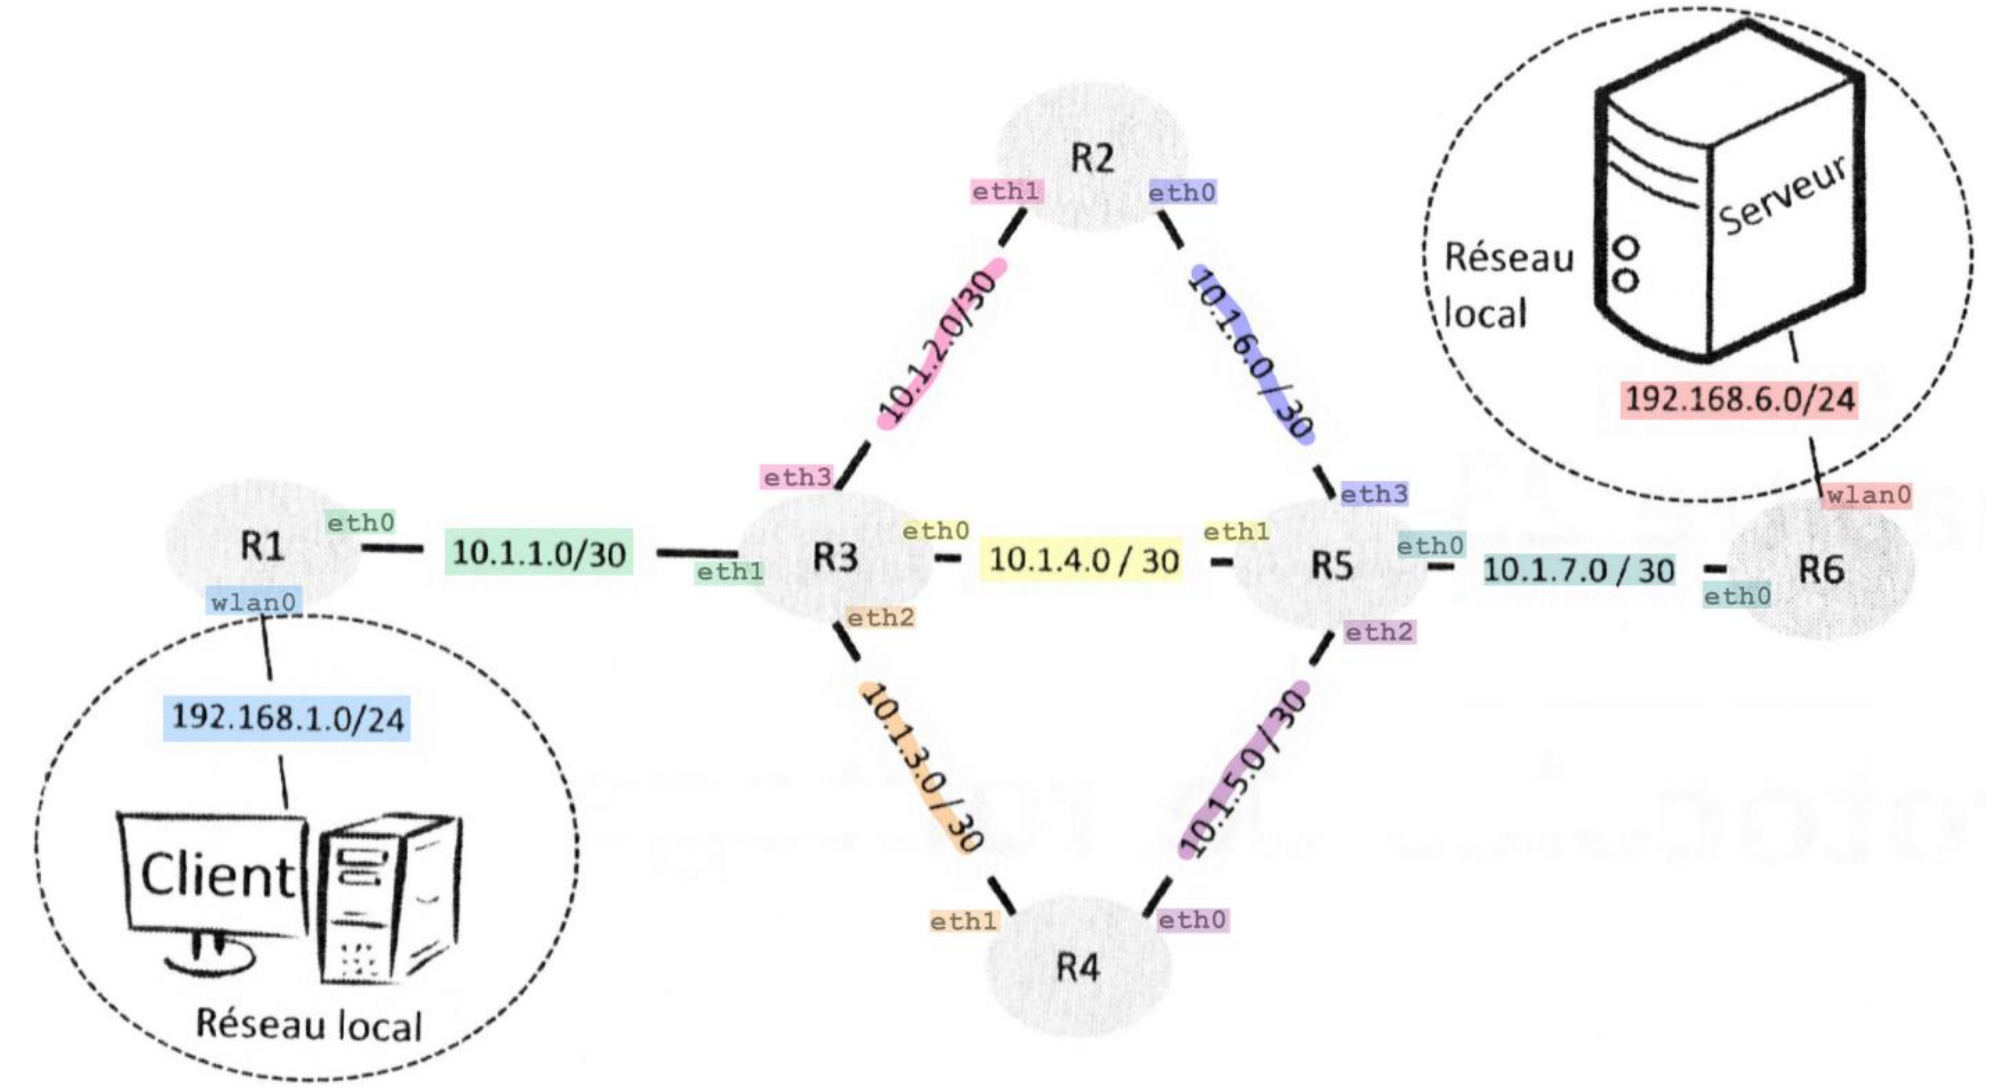
\includegraphics[width=10cm]{ressources/reseau.png}
\begin{aretenir}[Remarque]
Les interfaces (adresses entrées/sorties) des routeurs sont représentées par le type de connexion.
\end{aretenir}
\end{frame}

\begin{frame}
    \frametitle{Phase d'initialisation}
        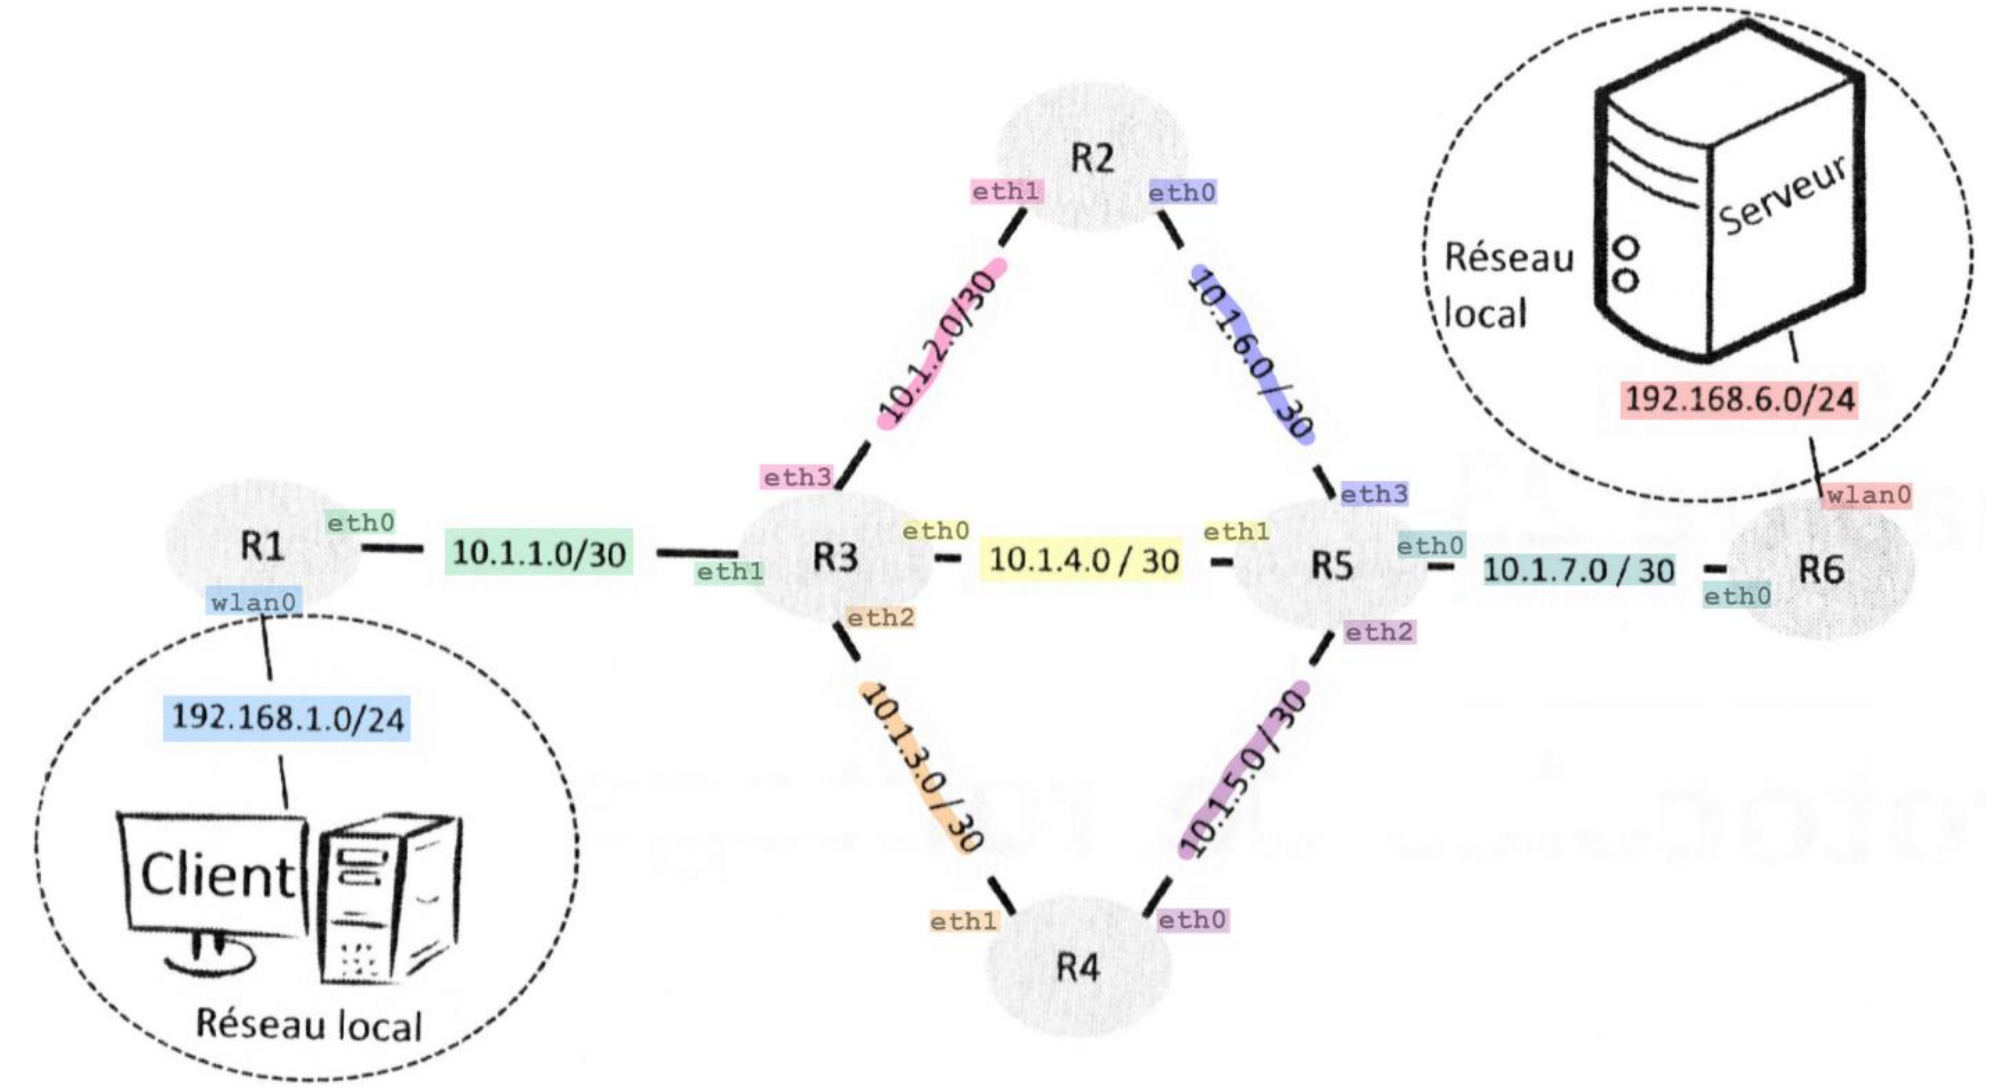
\includegraphics[width=9cm]{ressources/reseau.png}
\textbf{Phase d'initialisation (démarrage):} Le routeur récupère les informations de ses voisins immédiats.

        \begin{center}
    \begin{tabular}{|*{4}{c|}}
        \hline
        destination    & passerelle & interface & distance \\
        \hline
        10.1.1.0/30    &            & eth0      & 1        \\
        \hline
        192.168.1.0/24 &            & wlan0     & 1        \\
        \hline
    \end{tabular}
    \captionof{table}{Table de routage de R1}
\end{center}
\note{On atteint des réseaux (pas des routeurs) $\rightarrow$ passerelle vide pour les réseaux voisins.}
\end{frame}

\begin{frame}
    \frametitle{}
    \begin{center}
        \centering
        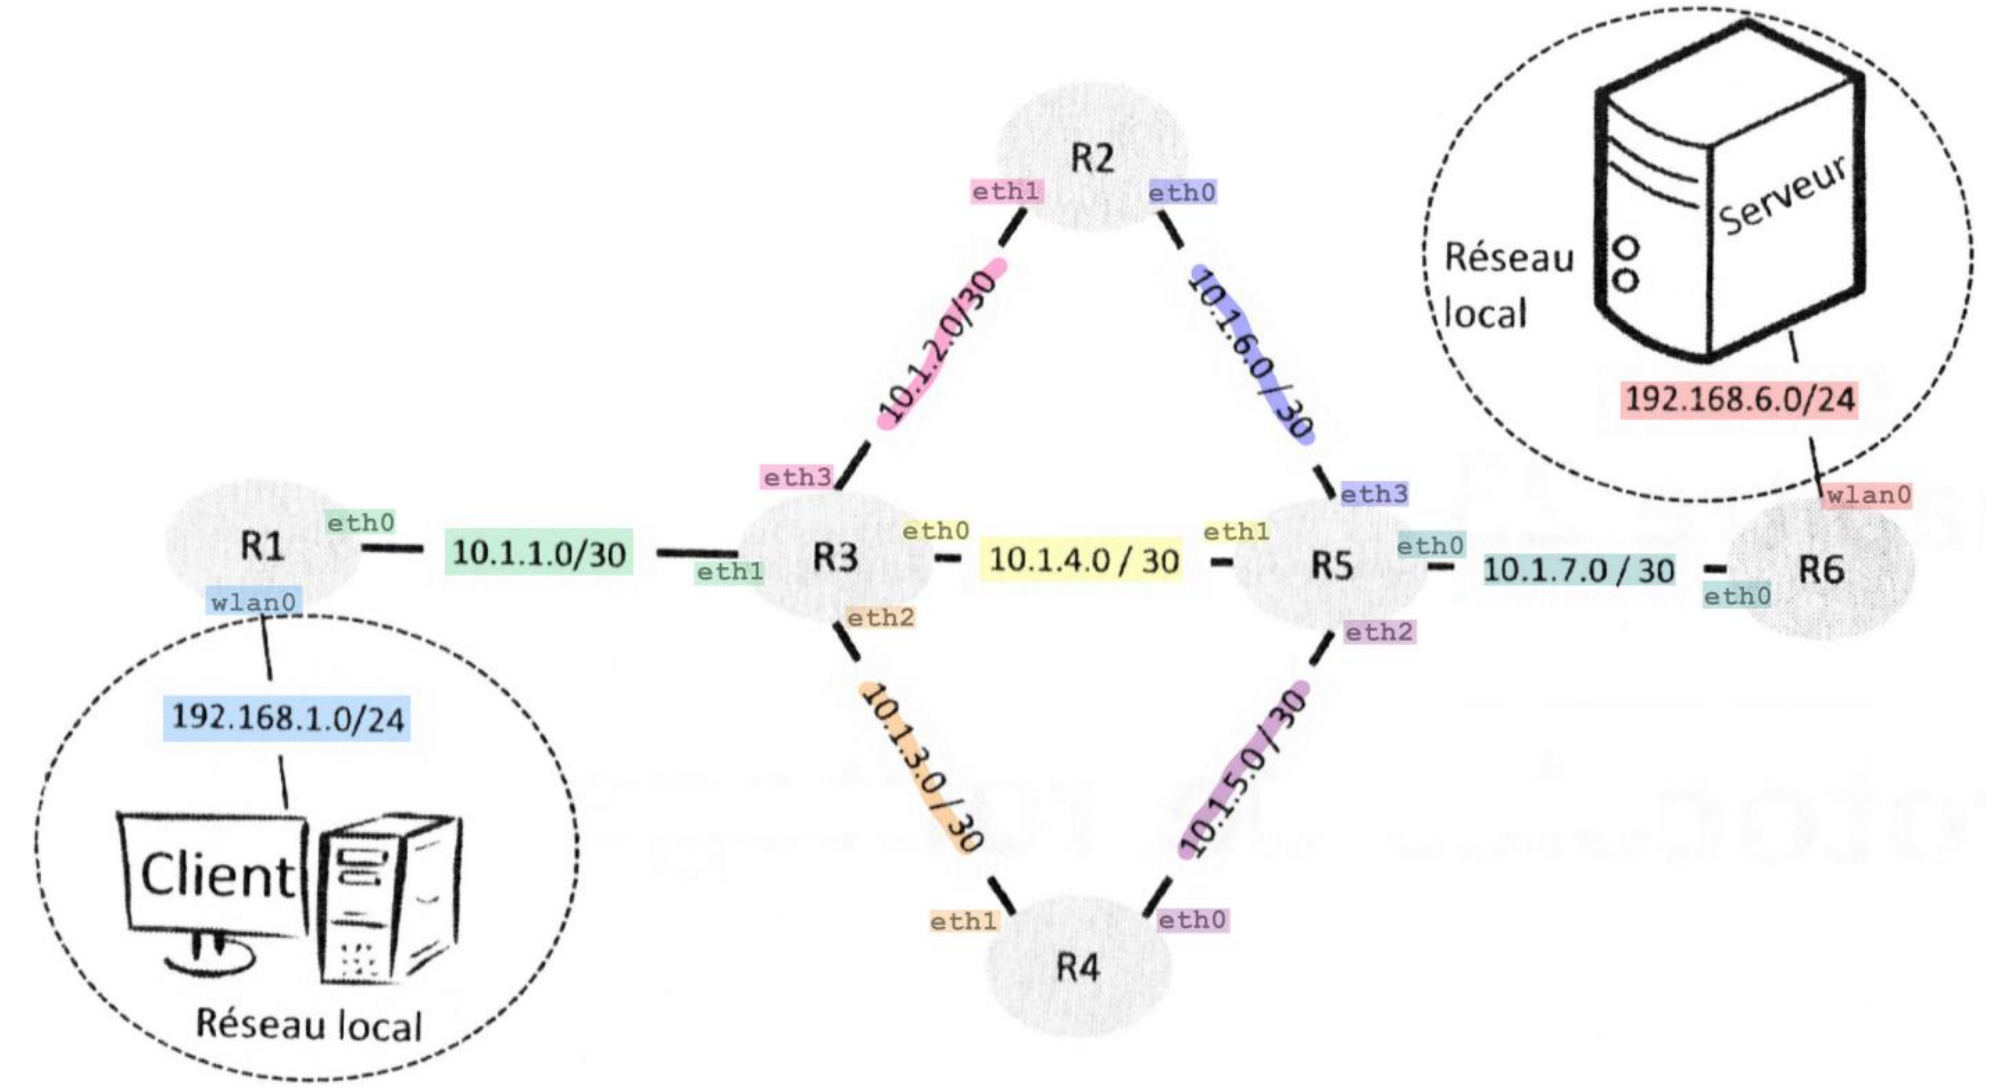
\includegraphics[width=10cm]{ressources/reseau.png}
        \captionof{figure}{Topologie du réseau}
        \label{reseau}
    \end{center}
    \begin{activite}
        Construire la table de routage du routeur R3 lors de la phase d'initialisation.
    \end{activite}

\end{frame}

\begin{frame}
    \frametitle{Correction}

    \begin{center}
        \begin{tabular}{|*{4}{c|}}
            \hline
            destination    & passerelle & interface & distance \\
            \hline
            10.1.1.0/30    &            & eth1      & 1        \\
            \hline
            10.1.2.0/30    &            & eth3      & 1        \\
            \hline
            10.1.3.0/30    &            & eth2      & 1        \\
            \hline
            10.1.4.0/30    &            & eth0      & 1        \\
            \hline
        \end{tabular}
        \captionof{table}{Table de routage de R3}
    \end{center}

\end{frame}

\begin{frame}
    \frametitle{Demande RIP}
    \begin{center}
        Lorsqu'un routeur reçoit une demande il accuse réception en renvoyant sa table de routage. Il existe alors plusieurs cas de figure.
    \end{center}
    \begin{itemize}
        \item<1-> Il découvre une nouvelle route
        \note[item]{vers un sous-réseau qui lui était jusque-là inconnu : il l’inscrit dans sa table.}
        \item<2-> Il découvre une route plus courte
        \note[item]{vers un sous-réseau connu mais passant par un autre routeur : il efface l’ancienne route de sa table et inscrit la nouvelle.}
        \item<3-> Il reçoit une nouvelle route plus longue \note[item]{il l’ignore.}
        \item<4-> Il reçoit une route existante, mais plus longue, vers un routeur passant par le même voisin. \note[item]{Cela veut dire qu’un problème est apparu sur son ancienne route. Il met donc à jour sa table avec cette nouvelle route. Pas représentatif sur cet exemple}
    \end{itemize}

\end{frame}
\begin{frame}
    \frametitle{}

    \begin{center}
        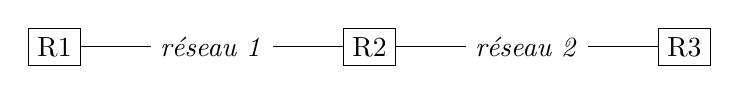
\begin{tikzpicture}
            \node[draw] (R1) at(0,0) {R1};
            \node[draw] (R2) at(4,0) {R2};
            \node[draw] (R3) at(8,0) {R3};
            \draw (R1) -- (R2) node[midway,fill=white]{\emph{réseau 1}};
            \draw (R2) -- (R3) node[midway,fill=white]{\emph{réseau 2}};
    
        \end{tikzpicture}
        \captionof{figure}{R1 découvre une route vers le réseau 2.}
    \end{center}
\begin{center}
    Il découvre une nouvelle route vers un sous-réseau qui lui était jusque-là inconnu : il l’inscrit dans sa table.
\end{center}
\end{frame}
\begin{frame}
    \frametitle{}

    \begin{center}
        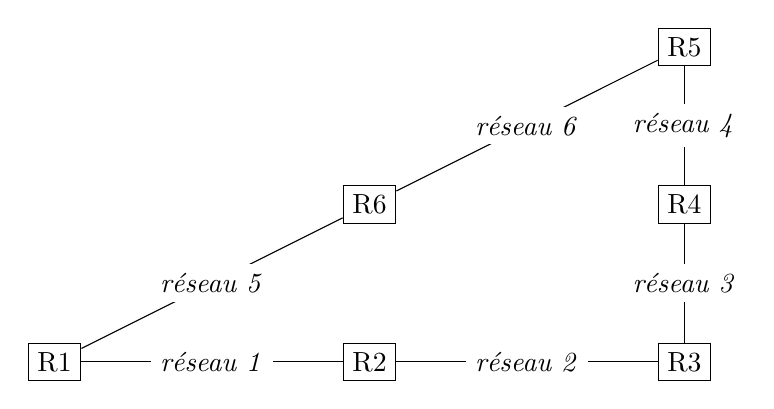
\begin{tikzpicture}
            \node[draw] (R1) at(0,0) {R1};
            \node[draw] (R2) at(4,0) {R2};
            \node[draw] (R3) at(8,0) {R3};
            \node[draw] (R4) at(8,2) {R4};
            \node[draw] (R5) at(8,4) {R5};
            \node[draw] (R6) at(4,2) {R6};

            \draw (R1) -- (R2) node[midway,fill=white]{\emph{réseau 1}};
            \draw (R2) -- (R3) node[midway,fill=white]{\emph{réseau 2}};
            \draw (R3) -- (R4) node[midway,fill=white]{\emph{réseau 3}};
            \draw (R4) -- (R5) node[midway,fill=white]{\emph{réseau 4}};
            \draw (R6) -- (R1) node[midway,fill=white]{\emph{réseau 5}};
            \draw (R6) -- (R5) node[midway,fill=white]{\emph{réseau 6}};
        \end{tikzpicture}
        \captionof{figure}{\centering R1 découvre une route plus courte vers le réseau 4, en passant par R6.}
    \end{center}
\begin{center}
    Il découvre une route plus courte vers un sous-réseau connu mais passant par un autre routeur : il efface l’ancienne route de sa table et inscrit la nouvelle.
    \note{ici on suppose que R1 connaissait déjà la route vers le réseau 4 en passant par R2.}
\end{center}
\end{frame}
\begin{frame}
    \frametitle{}

    \begin{center}
        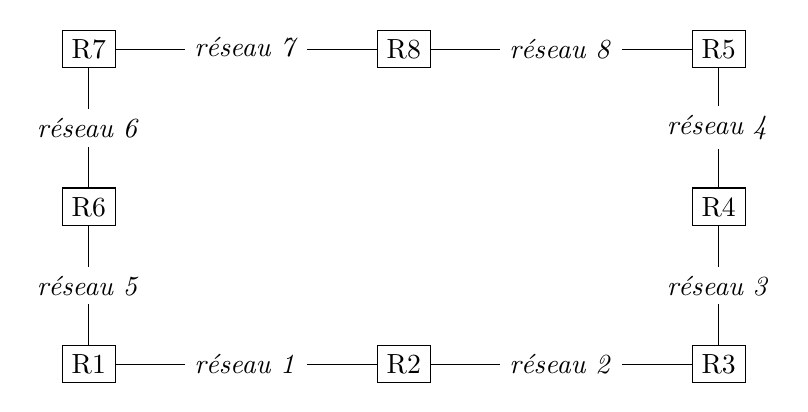
\begin{tikzpicture}
            \node[draw] (R1) at(0,0) {R1};
            \node[draw] (R2) at(4,0) {R2};
            \node[draw] (R3) at(8,0) {R3};
            \node[draw] (R4) at(8,2) {R4};
            \node[draw] (R5) at(8,4) {R5};
            \node[draw] (R6) at(0,2) {R6};
            \node[draw] (R7) at(0,4) {R7};
            \node[draw] (R8) at(4,4) {R8};

            \draw (R1) -- (R2) node[midway,fill=white]{\emph{réseau 1}};
            \draw (R2) -- (R3) node[midway,fill=white]{\emph{réseau 2}};
            \draw (R3) -- (R4) node[midway,fill=white]{\emph{réseau 3}};
            \draw (R4) -- (R5) node[midway,fill=white]{\emph{réseau 4}};
            \draw (R6) -- (R1) node[midway,fill=white]{\emph{réseau 5}};
            \draw (R6) -- (R7) node[midway,fill=white]{\emph{réseau 6}};
            \draw (R8) -- (R7) node[midway,fill=white]{\emph{réseau 7}};
            \draw (R8) -- (R5) node[midway,fill=white]{\emph{réseau 8}};
        \end{tikzpicture}
        \captionof{figure}{\centering R1 découvre une route plus longue vers le réseau 4, en passant par R6.}
    \end{center}
\begin{center}
    Il découvre une route plus longue vers un sous-réseau connu mais passant par un autre routeur : il l'ignore.
    \note{ici on suppose que R1 connaissait déjà la route vers le réseau 4 en passant par R2.}
\end{center}
\end{frame}
\begin{frame}
    \frametitle{}

    \begin{center}
        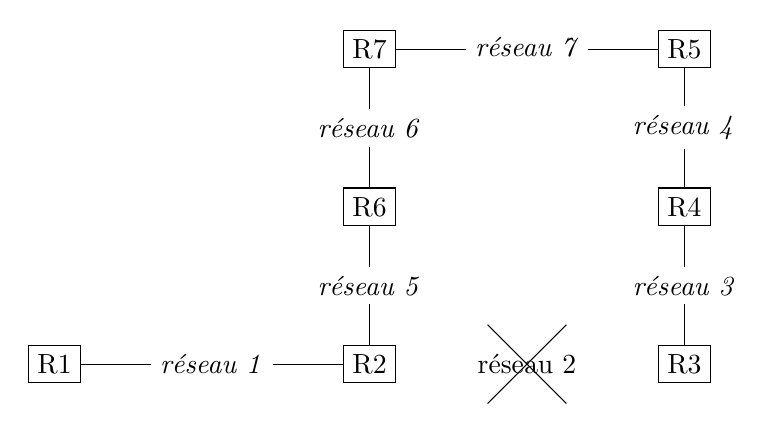
\begin{tikzpicture}
            \node[draw] (R1) at(0,0) {R1};
            \node[draw] (R2) at(4,0) {R2};
            \node[draw] (R3) at(8,0) {R3};
            \node[draw] (R4) at(8,2) {R4};
            \node[draw] (R5) at(8,4) {R5};
            \node[draw] (R6) at(4,2) {R6};
            \node[draw] (R7) at(4,4) {R7};

            \node at(6,0){réseau 2};
            \draw (5.5,0.5)--(6.5,-0.5);
            \draw (5.5,-0.5)--(6.5,0.5);

            \draw (R1) -- (R2) node[midway,fill=white]{\emph{réseau 1}};
            
            \draw (R3) -- (R4) node[midway,fill=white]{\emph{réseau 3}};
            \draw (R4) -- (R5) node[midway,fill=white]{\emph{réseau 4}};
            \draw (R6) -- (R2) node[midway,fill=white]{\emph{réseau 5}};
            \draw (R6) -- (R7) node[midway,fill=white]{\emph{réseau 6}};
            \draw (R7) -- (R5) node[midway,fill=white]{\emph{réseau 7}};
        \end{tikzpicture}
        \captionof{figure}{\centering R1 découvre une route plus longue vers le réseau 4, en passant par R2.}
    \end{center}
\begin{center}
    Il découvre une route existante, mais plus longue, vers un routeur passant par le même voisin: Cela signifie qu’un problème est apparu sur son ancienne route. Il met donc à jour sa table avec cette nouvelle route.
\end{center}
\end{frame}
\begin{frame}
    \frametitle{}

    \begin{aretenir}[Remarque]
        Lorsqu’un routeur reçoit une route, il augmente la distance associée à cette route de 1 pour prendre en compte le fait que les paquets devront passer par lui.
    \end{aretenir}

\end{frame}
\begin{frame}
    \frametitle{}

    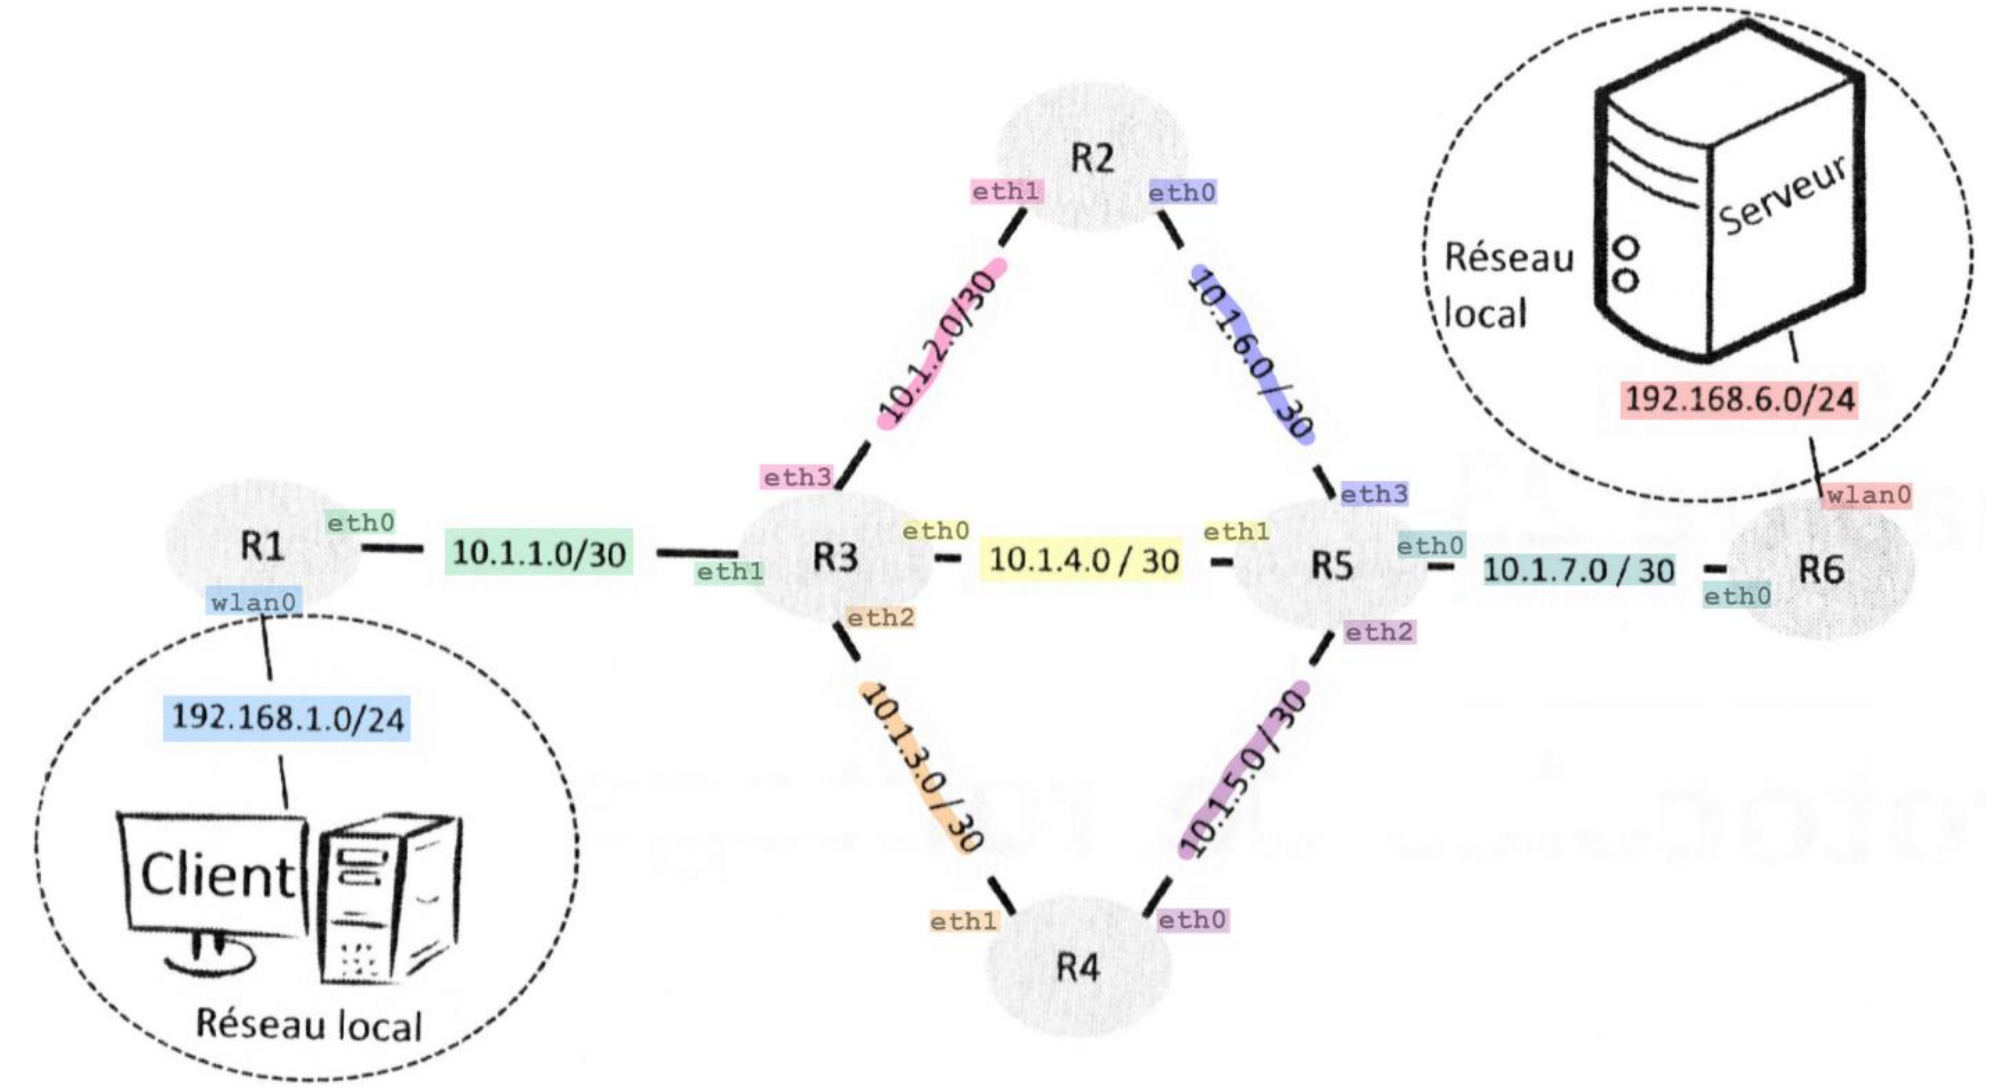
\includegraphics[width=10cm]{ressources/reseau.png}

\end{frame}
\begin{frame}
    \frametitle{}

    \begin{center}
        \begin{tabular}{|*{4}{c|}}
            \hline
            destination    & passerelle & interface & distance \\
            \hline
            10.1.1.0/30    &            & eth0      & 1        \\
            \hline
            192.168.1.0/24 &            & wlan0     & 1        \\
            \hline
            10.1.2.0/30    & R3         & eth0      & 2        \\
            \hline
            10.1.3.0/30    & R3         & eth0      & 2        \\
            \hline
            10.1.4.0/30    & R3         & eth0      & 2        \\
            \hline
        \end{tabular}
        \captionof{table}{Table de routage de R1 après son échange avec R3}
    \end{center}
\note{On pourrait noter l'interface du routeur voisin dans \emph{passerelle}.}
\end{frame}
\begin{frame}
    \frametitle{}

    \begin{activite}
        \begin{enumerate}
            \item Construire la table de routage de R3 après son échange avec R1.
            \item Construire la table de routage de R5 lors de la phase d'initialisation.
            \item Construire ensuite la table de routage de R3 après son échange avec R5.
        \end{enumerate}
    \end{activite}

\end{frame}
\begin{frame}
    \frametitle{Correction}

    \begin{center}
        \begin{tabular}{|*{4}{c|}}
            \hline
            destination    & passerelle & interface & distance \\
            \hline
            10.1.1.0/30    &            & eth1      & 1        \\
            \hline
            10.1.2.0/30    &            & eth3      & 1        \\
            \hline
            10.1.3.0/30    &            & eth2      & 1        \\
            \hline
            10.1.4.0/30    &            & eth0      & 1        \\
            \hline
            192.168.1.0/24    &     R1       & eth1      & 2        \\
            \hline
        \end{tabular}
        \captionof{table}{Table de routage de R3}
    \end{center}

\end{frame}

\begin{frame}
    \frametitle{Correction}

    \begin{center}
        \begin{tabular}{|*{4}{c|}}
            \hline
            destination    & passerelle & interface & distance \\
            \hline
            10.1.7.0/30    &            & eth0      & 1        \\
            \hline
            10.1.6.0/30    &            & eth3      & 1        \\
            \hline
            10.1.5.0/30    &            & eth2      & 1        \\
            \hline
            10.1.4.0/30    &            & eth1      & 1        \\
            \hline
        \end{tabular}
        \captionof{table}{Initialisation de R5}
    \end{center}

\end{frame}

\begin{frame}
    \frametitle{Correction}

    \begin{center}
        \begin{tabular}{|*{4}{c|}}
            \hline
            destination    & passerelle & interface & distance \\
            \hline
            10.1.7.0/30    &            & eth0      & 1        \\
            \hline
            10.1.6.0/30    &            & eth3      & 1        \\
            \hline
            10.1.5.0/30    &            & eth2      & 1        \\
            \hline
            10.1.4.0/30    &            & eth1      & 1        \\
            \hline
            10.1.1.0/30    &      R3      & eth1      & 2        \\
            \hline
            10.1.2.0/30    &     R3       & eth1      & 2        \\
            \hline
            10.1.3.0/30    &       R3     & eth1      & 2        \\
            \hline
            192.168.1.0/24    &     R3       & eth1      & 3        \\
            \hline
        \end{tabular}
        \captionof{table}{Table de routage de R5 après son échange avec R3}
    \end{center}
\note[item]{les échanges ne sont pas forcément synchrones: si R5 a échangé avec R2 avant, le chemin vers 10.1.2.0 serait différent}

\end{frame}
\begin{frame}
    \frametitle{}

    \begin{aretenir}[Remarque]
        Au bout de quelques échanges les tables sont stabilisées: les routeurs connaissent toutes les routes.
    \end{aretenir}

\end{frame}
\section{Gestion des pannes}
\begin{frame}
    \frametitle{Gestion des pannes}

    \begin{itemize}
        \item\textbf{15 sauts maximum:} au-delà la route est oubliée.
        \note[item]{également si un routeur ne reçoit pas d'information de la part d'un de ses voisins au
        bout d'un certain laps de temps (par défaut, 3 minutes (configurable)), il va considérer que ce
        lien est mort et en informer ses voisins en indiquant un nombre de sauts égal à 16.}
        \note[item]{délai de convergence = temps pour que tous les routeurs aient la même vue de la topologie $\rightarrow$ 15 sauts permet de réduire ce délai}
    \end{itemize}

\end{frame}

\begin{frame}
    \frametitle{}

    \begin{itemize}
        \item\textbf{split horizon:} un routeur ne renvoie pas une information à un autre routeur s’il a appris cette information par ce même routeur.
    \end{itemize}
\begin{center}
\centering
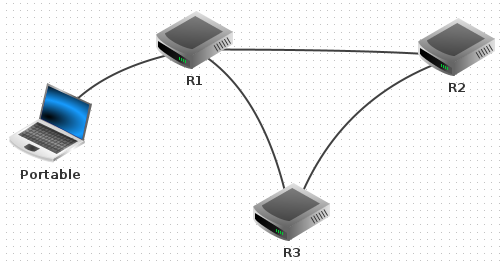
\includegraphics[width=8cm]{ressources/split.png}
\captionof{figure}{Boucle de routage}
\label{IMG}
\end{center}
\end{frame}

\begin{frame}
    \frametitle{Split horizon}

    \begin{center}
        \centering
        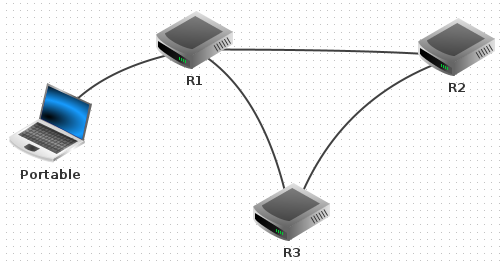
\includegraphics[width=6cm]{ressources/split.png}
        \captionof{figure}{Boucle de routage}
        \label{IMG}
        \end{center}
Supposons une défaillance qui rend le réseau du portable inaccessible: R1 note une métrique infinie (16) vers ce réseau.
\end{frame}
\begin{frame}
    \frametitle{Split horizon}

    \begin{center}
        \centering
        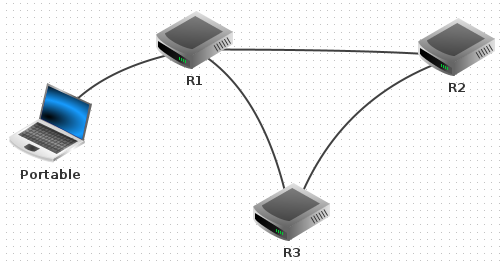
\includegraphics[width=6cm]{ressources/split.png}
        \captionof{figure}{Boucle de routage}
        \label{IMG}
        \end{center}
R1 envoie cette information à R2\dots mais en même temps R2 envoie une route vers le réseau du portable avec une métrique de 3.
\note{les envois ne sont pas forcément synchrones.}
\end{frame}

\begin{frame}
    \frametitle{Split horizon}

    \begin{center}
        \centering
        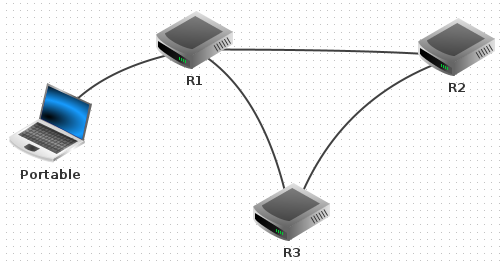
\includegraphics[width=6cm]{ressources/split.png}
        \captionof{figure}{Boucle de routage}
        \label{IMG}
        \end{center}
À la mise à jour suivante, R2 communiquera une métrique infinie mais R1 renverra une métrique de 4 $$\downarrow$$ \begin{center}
    boucle de réseau
\end{center}
\note[item]{R1 à incrémenter de 1}
\note[item]{C'est cette étape qui est bloquée par le split horizon: R1 ne renvoie pas à R2}
\end{frame}

\begin{frame}
    \frametitle{}

    \begin{itemize}
        \item\textbf{hold down:} lorsqu'un routeur prend connaissance de l'indisponibilité d'une route vers un sous-réseau, il doit ignorer toute information concernant un chemin vers ce sous réseau pendant une durée égale au \emph{temporisateur (hold down)}.
    \end{itemize}
\note{Avec cette fonction, le temps est laissé à l'information d'indisponibilité de la route à se communiquer à tous les routeurs.}
\end{frame}
\begin{frame}
    \frametitle{}

    \begin{aretenir}[Remarque]
        La limite de 15 sauts ne permet pas d'utiliser ce protocole pour de grands réseaux.
    \end{aretenir}

\end{frame}
\end{document}